\documentclass[11pt,letterpaper]{article}
\usepackage[top=3cm, bottom=2cm, left=2cm, right=2cm, columnsep=20pt]{geometry}
\usepackage{pdfpages}
\usepackage{graphicx}
\usepackage{etoolbox}
\apptocmd{\sloppy}{\hbadness 10000\relax}{}{}
% \usepackage[numbers]{natbib}
\usepackage[T1]{fontenc}
\usepackage{ragged2e}
\usepackage[french]{babel}
\usepackage{listings}
\usepackage{color}
\usepackage{soul}
\usepackage[utf8]{inputenc}
\usepackage[export]{adjustbox}
\usepackage{caption}
\usepackage{amsmath}
\usepackage{amssymb}
\usepackage{float}
\usepackage{csquotes}
\usepackage{fancyhdr}
\usepackage{wallpaper}
\usepackage{siunitx}
\usepackage[indent]{parskip}
\usepackage{textcomp}
\usepackage{gensymb}
\usepackage{multirow}
\usepackage[hidelinks]{hyperref}
\usepackage{abstract}
\usepackage{svg}
\usepackage{biblatex}
\addbibresource{bibliographie.bib}

\renewcommand{\abstractnamefont}{\normalfont\bfseries}
\renewcommand{\abstracttextfont}{\normalfont\itshape}
\usepackage{titlesec}
\titleformat{\section}{\large\bfseries}{\thesection}{1em}{}
\titleformat{\subsection}{\normalsize\bfseries}{\thesubsection}{1em}{}
\titleformat{\subsubsection}{\normalsize\bfseries}{\thesubsubsection}{1em}{}

\usepackage{xcolor}
\definecolor{codegreen}{rgb}{0,0.6,0}
\definecolor{codegray}{rgb}{0.5,0.5,0.5}
\definecolor{codepurple}{rgb}{0.58,0,0.82}
\definecolor{backcolour}{rgb}{0.95,0.95,0.92}
\lstdefinestyle{mystyle}{
    backgroundcolor=\color{backcolour},   
    commentstyle=\color{codegreen},
    keywordstyle=\color{magenta},
    numberstyle=\tiny\color{codegray},
    stringstyle=\color{codepurple},
    basicstyle=\ttfamily\footnotesize,
    breakatwhitespace=false,         
    breaklines=true,                 
    captionpos=b,                    
    keepspaces=true,                 
    numbers=left,                    
    numbersep=5pt,                  
    showspaces=false,                
    showstringspaces=false,
    showtabs=false,                  
    tabsize=2
}
\lstset{style=mystyle}

\usepackage[most]{tcolorbox}
\newtcolorbox{note}[1][]{
  enhanced jigsaw,
  borderline west={2pt}{0pt}{black},
  sharp corners,
  boxrule=0pt, 
  fonttitle={\large\bfseries},
  coltitle={black},
  title={Note:\ },
  attach title to upper,
  #1
}

%----------------------------------------------------

\setlength{\parindent}{0pt}
\DeclareCaptionLabelFormat{mycaptionlabel}{#1 #2}
\captionsetup[figure]{labelsep=colon}
\captionsetup{labelformat=mycaptionlabel}
\captionsetup[figure]{name={Figure }}
\newcommand{\inlinecode}{\normalfont\texttt}
\usepackage{enumitem}
\setlist[itemize]{label=\textbullet}

\begin{document}
\begin{titlepage}
\center

\begin{figure}
    \ThisULCornerWallPaper{.4}{Polytechnique_signature-RGB-gauche_FR.png}
\end{figure}
\vspace*{2 cm}

\textsc{\Large \textbf{PHS3910 --} Techniques expérimentales et instrumentation}\\[0.5cm]
\large{\textbf{Équipe : Lundi 03}}\\[1.5cm]

\rule{\linewidth}{0.5mm} \\[0.5cm]
\Large{\textbf{Spectromètre}} \\[0.2cm]
\text{Fiche technique}\\
\rule{\linewidth}{0.2mm} \\[2.3cm]

\large{\textbf{Présenté à}\\
  Jean Provost\\
  Lucien Weiss\\[2.5cm]
  \textbf{Par :}\\
  Émile \textbf{Guertin-Picard} (2208363)\\
  Philippine \textbf{Beaubois} (2211153)\\
  Marie-Lou \textbf{Dessureault} (2211129)\\
  Maxime \textbf{Rouillon} (2213291)\\[3cm]}

\large{\today\\
Département de Génie Physique\\
Polytechnique Montréal\\}

\end{titlepage}

%----------------------------------------------------

\tableofcontents
\pagenumbering{roman}
\newpage

\pagestyle{fancy}
\setlength{\headheight}{14pt}
\renewcommand{\headrulewidth}{0pt}
\fancyfoot[R]{\thepage}

\pagestyle{fancy}
\fancyhf{}
\renewcommand{\headrulewidth}{1pt}
\fancyhead[L]{\textbf{PHS3910}}
\fancyhead[C]{Fiche technique des spectromètres}
\fancyhead[R]{\today}
\fancyfoot[R]{\thepage}

\pagenumbering{arabic}
\setcounter{page}{1}

%----------------------------------------------------

\section{Description générale et spécifications}

Cette fiche technique présente les caractéristiques de deux spectromètres : l'un construit sur 
table optique et l'autre avec de l'impression 3D. Pour les deux appareils, le même système 4f
est construit. La lumière passe au travers d'une fente de taille \textcolor{red}{XX} mm, 
ajustable sur la table optique (VA100), ou faite avec des lames de rasoir parallèles pour le
système imprimé. Cette lumière est convergée avec une lentille de distance focale de 50 mm 
(LA-1213-A-ML) sur un réseau de diffraction blazé à 600 rainures/mm (GR25-0605) placé à un
angle de \textcolor{red}{XX}\degree $\;$afin que la réflexion d'ordre 1 qui sépare les
longueurs d'onde spatialement soit renvoyée vers une deuxième lentille de distance focale
de 25 mm (LA-1560-A-ML). Cette réflexion, au travers de la lentille, place le spectre des 
longueurs d'ondes sur le capteur d'une caméra (DCC1545M-GL) pour l'analyse. Les deux appareils
sont concus pour que la caméra capte entre 397 nm et 666 nm. Le modèle imprimé présente une
résolution de \textcolor{red}{XX $\pm$ XX} nm et un coût total de 877.28\$. Le modèle sur
table optique a une résolution de \textcolor{red}{XX $\pm$ XX} nm et coûte 1852.72\$. Les
deux spectromètres et leurs dimensions physiques sont présentés à la figure 
\ref{schema_spectros} :


\begin{figure}[H]
  \centering
  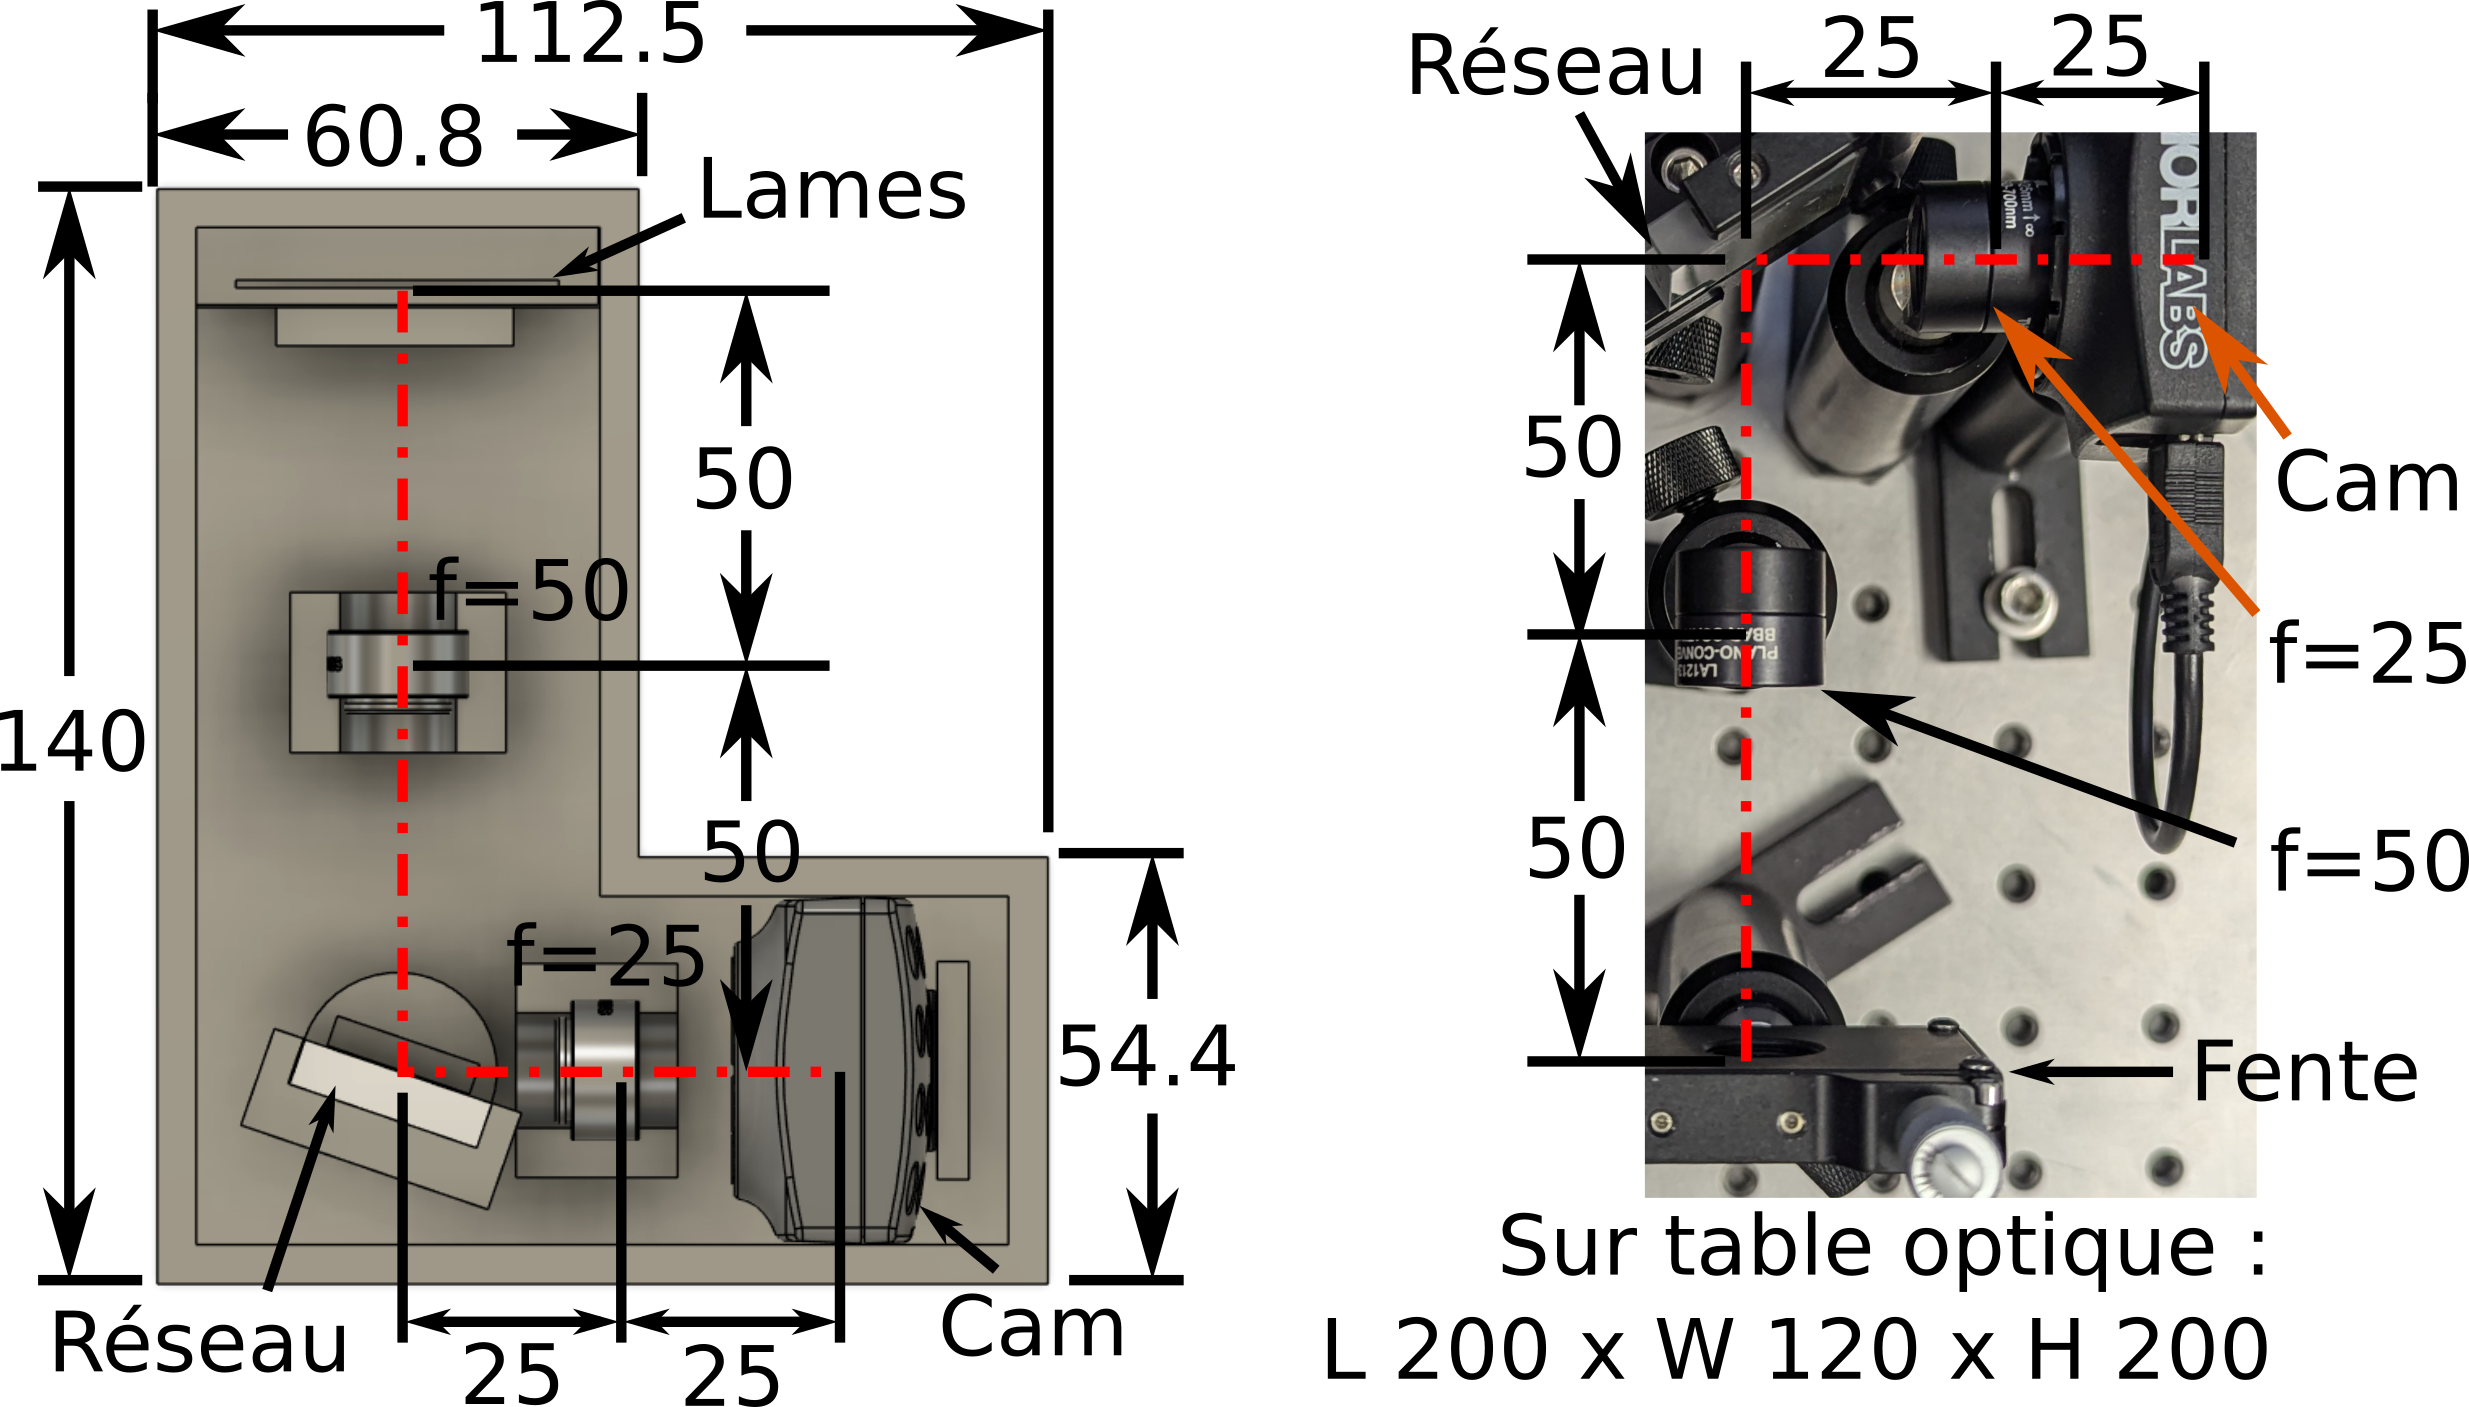
\includegraphics[scale=1.75]{schema_spectros.png}
  \caption{Schémas des spectromètres. Toutes les dimensions sont en millimètres. À gauche : spectromètre fait par impression 3D sans son couvercle. À droite : spectromètre sur table optique.}
  \label{schema_spectros}
\end{figure}


\section{Rapports de tests}

L'objectif primaire de la construction de deux spectromètres séparés est de permettre la 
comparaison des coûts et de la performance des deux dispositifs. Cette section présente
donc les tests qui ont été effectués pour caractériser les dispositifs, et présente les 
conclusions quant à la performance des dispositifs.

\subsection{Caractérisation de la résolution}

\textcolor{red}{plz détailler comment la méthode de comment trouver la résolution}

\subsection{Rapport détaillé des coûts}

Les méthodes de construction étant grandement différentes pour les deux spectromètres, une 
étude des coûts est faite afin de déterminer lequel des deux est le plus abordable. Pour ce
faire, une liste détaillée des pièces requises est faite, et le total des coûts est calculé en
dollars canadiens avant taxes. La table \ref{prix_table} présente les coûts des pièces pour
le système monté sur table optique :

\begin{table}[!ht]
    \centering
    \caption{Liste des pièces et coûts totaux pour le spectromètre sur table optique}
    \begin{tabular}{|l|l|c|r|r|}
    \hline
        ID pièce & Description & Qté & \$ CAD & Total ind. \\ \hline\hline
        LA-1560-A-ML & Lentille plano-convexe f=25 mm & 1 & \$72.25 & \$72.25 \\ \hline
        LA-1213-A-ML & Lentille plano-convexe f=50 mm & 1 & \$70.61 & \$70.61 \\ \hline
        NE506A & Filtre atténuateur de lumière & 2 & \$59.55 & \$119.10 \\ \hline
        GR25-0605 & Réseau de diffraction 600/mm & 1 & \$178.32 & \$178.32 \\ \hline
        DCC1545M-GL & Caméra USB & 1 & \$539.21 & \$539.21 \\ \hline
        VA100 & Fente ajustable & 1 & \$417.74 & \$417.74 \\ \hline
        KM100S & Montage à réseau de diffraction & 1 & \$130.45 & \$130.45 \\ \hline
        SMR05 & Trou taraudé pour lentilles & 2 & \$28.68 & \$57.35 \\ \hline
        TR3-P5, & 5 tiges pour optiques & 1 & \$38.50 & \$38.50 \\ \hline
        BA1 & Pied de montage optique & 2 & \$8.42 & \$16.85 \\ \hline
        BA1S & Pied de montage optique & 4 & \$7.83 & \$31.30 \\ \hline
        PH6 & Base pour tiges d'optique & 5 & \$20.43 & \$102.17 \\ \hline
        PH4 & Base pour tiges d'optique & 1 & \$14.83 & \$14.83 \\ \hline
        VC1 & Pince en V & 1 & \$64.04 & \$64.04 \\ \hline\hline
        ~ & ~ & ~ & Total : & \$1,852.72 \\ \hline
    \end{tabular}
    \label{prix_table}
\end{table}

Quelques points sont à relever pour cette table. La caméra utilisée est maintenant indisponible
à l'achat sur le site de Thorlabs. Le prix affiché est donc le prix de cette pièce avant
qu'elle soit enlevée du site en 2021 \textcolor{red}{source A}. Aussi, deux éléments importants
ont été omis de cette liste. La quincaillerie, soit les vis, les écrous et les 
rondelles, n'ont pas été comptées car ces derniers sont fréquemment disponibles en vrac dans
des ateliers, ou ils s'achètent en ensemble à moindre coût. La table pour fixer les éléments 
optiques n'a pas été comptée non plus car elle ne servait pas que pour le spectromètre 
construit. Sa taille, donc son prix est donc beaucoup trop grand par rapport au besoin du projet. L'appareil
construit fonctionnerait sur la table B1212F, mesurant 12 x 12 po. Avec un coût de 966.85\$,
le total serait amené à 2819.57\$. L'achat de cette table pourrait toutefois ne pas être 
justifiable pour un laboratoire étant donné sa taille restreinte, donc des options plus grandes
seraient à considérer.

% source A : https://www.thorlabs.com/thorProduct.cfm?partNumber=DCC1545M

La table \ref{prix_3D} montre le calcul des coûts pour le modèle fait par l'impression 3D :

\begin{table}[!ht]
    \centering
    \caption{Liste des pièces et coûts totaux pour le spectromètre avec impression 3D}
    \begin{tabular}{|l|l|c|r|r|}
    \hline
        ID pièce & Description & Qté & \$ CAD & Total ind. \\ \hline\hline
        LA-1560-A-ML & Lentille plano-convexe f=25 mm & 1 & \$72.25 & \$72.25 \\ \hline
        LA-1213-A-ML & Lentille plano-convexe f=50 mm & 1 & \$70.61 & \$70.61 \\ \hline
        GR25-0605 & Réseau de diffraction 600/mm & 1 & \$178.32 & \$178.32 \\ \hline
        DCC1545M-GL & Caméra USB & 1 & \$539.21 & \$539.21 \\ \hline
        - & Impression 3D & 1 & \$6.94 & \$6.94 \\ \hline
        - & Ensemble de lames de rasoir & 1 & \$9.95 & \$9.95 \\ \hline\hline
        ~ & ~ & ~ & Total : & \$877.28 \\ \hline
    \end{tabular}
    \label{prix_3D}
\end{table}

Un élément a aussi été exclu de cette liste, soit l'imprimante 3D utilisée pour l'impression.
Celle utilisée, soit la Original Prusa i3 MK3S+, est disponible pour 899\$ US, ou 1245.21\$ CAD.
Si considéré, ce prix augmente grandement les coûts associé à ce modèle de spectromètre, étant
plus dispendieux que le total calculé. Toutefois, ce type d'imprimante est facilement accessible
gratuitement en faisant affaire avec certains ateliers. Aussi, pour de faibles quantités de
pièces, il est possible de commander des impressions en ligne pour beaucoup moins cher que
l'imprimante. C'est donc pourquoi son prix a été omis.

Il est donc facile de conclure que l'impression 3D est beaucoup plus avantageux économiquement.
Le prix de l'impression sous 10\$ est une très grande économie lorsque comparé aux nombreuses
pièces servant au montage sur table optique qui ont fortement contribués au coût élevé du
modèle qui les requiert. L'économie de 975.44\$ en allant avec le modèle imprimé est
considérable, et appuie le fait que c'est le modèle à préconiser.



% \clearpage
% \printbibliography
% \bibliographystyle{unsrtnat}
% \bibliography{My_Library}

\end{document}
